\documentclass{beamer}
\usetheme{Madrid}
\usecolortheme{whale}
\usepackage{tikz}
\usetikzlibrary{shapes,arrows,positioning,fit,calc}
\usepackage{pgfplots}
\pgfplotsset{compat=1.18}
\usepackage{amsmath}
\usepackage{graphicx}

% Add footer template with logo on the left and slide numbers on the right
\setbeamertemplate{footline}{
  \leavevmode%
  \hbox{%
  \begin{beamercolorbox}[wd=.1\paperwidth,ht=2.25ex,dp=1ex,center]{date in head/foot}%
    \includegraphics[height=2ex]{ua_logo.png}
  \end{beamercolorbox}%
  \begin{beamercolorbox}[wd=.8\paperwidth,ht=2.25ex,dp=1ex,center]{title in head/foot}%
    \usebeamerfont{title in head/foot}\insertshorttitle
  \end{beamercolorbox}%
  \begin{beamercolorbox}[wd=.1\paperwidth,ht=2.25ex,dp=1ex,right]{date in head/foot}%
    \usebeamerfont{date in head/foot}\insertframenumber{}/\inserttotalframenumber\hspace*{2ex}
  \end{beamercolorbox}}%
  \vskip0pt%
}

\title{Clustering and Disjoint Principal Component Analysis (CDPCA) in Financial Markets}
\author[123155/123177/126784]{Syed Muhammad Zeeshan Bukhari ( 123155 )\\
Silvia Mastracci ( 123177 )\\
Oleksandr Solovei ( 126784 )
}
\date{\today}

\begin{document}

\begin{frame}
    \titlepage
\end{frame}

\begin{frame}{Introduction}
    \begin{block}{Problem Statement}
        \begin{itemize}
            \item High dimensionality of financial market data
            \item Complex correlations between market sectors
            \item Missing data in financial time series adds another layer of complexity
            \item Challenge in identifying distinct market patterns
        \end{itemize}
    \end{block}

    \begin{block}{Objectives}
        \begin{itemize}
            \item Apply CDPCA to financial market data
            \item Introduce a new element by integrating missing data handling into the CDPCA framework.
            \item Address the challenge of missing data using different techniques
            \item Identify disjoint components in market sectors
        \end{itemize}
    \end{block}
\end{frame}

\begin{frame}{Motivation}
    \begin{block}{Why CDPCA for Financial Markets?}
        \begin{itemize}
            \item Traditional PCA: Components can be hard to interpret due to mixed loadings
            \item K-means alone: Misses underlying market structure
            \item Need: Clear sector-based patterns for investment decisions
        \end{itemize}
    \end{block}

    \begin{block}{Key Advantages}
        \begin{itemize}
            \item Disjoint components: Each asset belongs to exactly one component
            \item Simultaneous clustering: Groups similar assets together
            \item Enhanced interpretability: Clear sector-based patterns
        \end{itemize}
    \end{block}
\end{frame}

\begin{frame}{CDPCA Model}
    \begin{block}{Mathematical Framework}
        \begin{equation*}
            \mathbf{X} = \mathbf{U}\hat{\mathbf{Y}}\mathbf{A}' + \mathbf{E}
        \end{equation*}
        where:
        \begin{itemize}
            \item $\mathbf{X}$: Matrix of asset returns $(I \times J)$
            \item $\mathbf{U}$: Asset cluster membership $(I \times P)$
            \item $\hat{\mathbf{Y}}$: Cluster centroids $(P \times Q)$
            \item $\mathbf{A}$: Component loading matrix transposed $(Q \times J)$
            \item $\mathbf{E}$: Error matrix $(I \times J)$
        \end{itemize}
    \end{block}
\end{frame}

\begin{frame}{CDPCA Algorithm}
    \begin{block}{Alternating Least Squares (ALS) Steps}
        \begin{enumerate}
            \item Update asset clusters ($\mathbf{U}$)
            \item Calculate cluster centroids ($\hat{\mathbf{Y}}$)
            \item Update component loadings ($\mathbf{A}$)
            \item Repeat until convergence
        \end{enumerate}
    \end{block}

    \begin{block}{Optimization Problem}
        Maximize between-cluster variance:
        \begin{equation*}
            \max_{\mathbf{U},\hat{\mathbf{Y}},\mathbf{A}} \|\mathbf{U}\hat{\mathbf{Y}}\mathbf{A}'\|^2
        \end{equation*}
        Subject to structural constraints
    \end{block}
\end{frame}


\begin{frame}{CDPCA Visualization: Process Flow}
    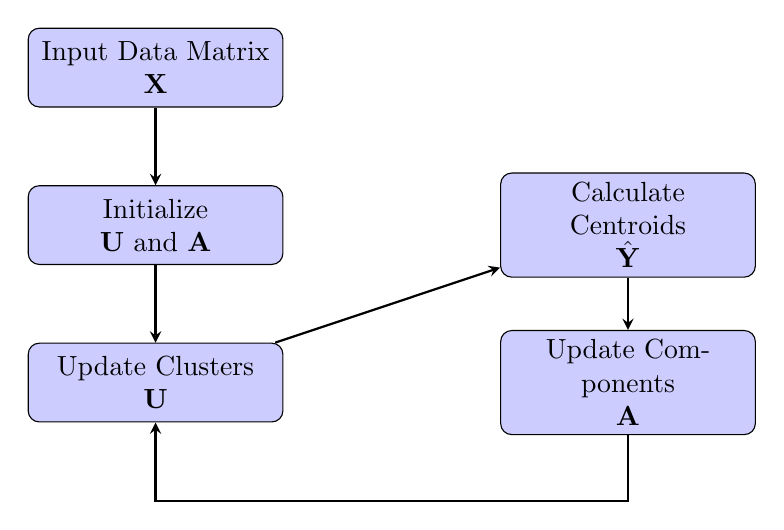
\begin{tikzpicture}[node distance=2cm]
        % Define styles
        \tikzstyle{block} = [rectangle, draw, fill=blue!20,
            text width=3cm, text centered, rounded corners, minimum height=1cm]
        \tikzstyle{arrow} = [thick,->,>=stealth]

        % Nodes
        \node [block] (data) {Input Data Matrix\\$\mathbf{X}$};
        \node [block, below of=data] (init) {Initialize\\$\mathbf{U}$ and $\mathbf{A}$};
        \node [block, below of=init] (cluster) {Update Clusters\\$\mathbf{U}$};
        \node [block, right of=cluster, xshift=4cm] (component) {Update Components\\$\mathbf{A}$};
        \node [block, above of=component] (centroid) {Calculate Centroids\\$\hat{\mathbf{Y}}$};

        % Arrows
        \draw [arrow] (data) -- (init);
        \draw [arrow] (init) -- (cluster);
        \draw [arrow] (cluster) -- (centroid);
        \draw [arrow] (centroid) -- (component);
        \draw [arrow] (component) -- ++(0,-1.5) -| (cluster);

    \end{tikzpicture}
\end{frame}

\begin{frame}{Data Overview}

    \begin{block}{Data Source and Structure}
        \begin{itemize}
            \item Source: Yahoo Finance (quantmod R)
            \item Period: 2022-01-01 to 2023-12-31 (252 trading days/year)
            \item Daily market data for 9 stocks
        \end{itemize}
    \end{block}

    \begin{block}{Variables and Properties}
        \begin{description}\setlength{\itemsep}{1pt}
            \item[Price] Open, High, Low, Close, Adjusted Close (adjusted for corporate actions)
            \item[Volume] Daily trading volume (number of shares traded)
        \end{description}
        \vspace{4mm}
        \begin{itemize}
            \item Data standardized, missing values removed
            \item Dimensions: Rows (trading days), Columns (6 variables)
        \end{itemize}
    \end{block}


\end{frame}


\begin{frame}{Data Structure \& Coverage}
    \begin{columns}
        % Left Column
        \begin{column}{0.48\textwidth}
            \begin{block}{Dataset Overview}
                \begin{itemize}
                    \item \textbf{Observations}: 4,509 total
                    \item \textbf{Period}: 501 trading days
                    \item \textbf{Variables}: 6 per stock
                    \item \textbf{Missing Values}: None after cleaning
                \end{itemize}
            \end{block}

            \begin{block}{Variable Statistics}
                \begin{itemize}\setlength{\itemsep}{0pt}
                    \item All variables standardized
                    \item \textbf{Volume Range}: -0.91 to 6.79
                    \item \textbf{Price Range}: -1.33 to 2.57
                    \item High correlations within price variables
                \end{itemize}
            \end{block}
        \end{column}

        % Right Column
        \begin{column}{0.48\textwidth}
            \begin{block}{Market Sectors}
                \textbf{Technology} (NASDAQ)
                \begin{itemize}\setlength{\itemsep}{0pt}
                    \item AAPL: Apple Inc
                    \item MSFT: Microsoft Corp
                    \item GOOGL: Alphabet Inc
                \end{itemize}
                \textbf{Finance} (NYSE)
                \begin{itemize}\setlength{\itemsep}{0pt}
                    \item JPM: JPMorgan Chase
                    \item V: Visa Inc
                    \item MA: Mastercard Inc
                \end{itemize}
                \textbf{Consumer} (NYSE)
                \begin{itemize}\setlength{\itemsep}{0pt}
                    \item KO: Coca-Cola Co
                    \item PG: Procter \& Gamble
                    \item WMT: Walmart Inc
                \end{itemize}
            \end{block}
        \end{column}
    \end{columns}
\end{frame}

\begin{frame}{Variable Structure}
   \begin{tikzpicture}
       \begin{axis}[
           width=\textwidth,
           height=0.7\textheight,
           xlabel=Variables,
           ylabel=Loading Values,
           title=CDPCA Variable Loadings,
           symbolic x coords={Open, High, Low, Close, Volume, Adjusted},
           xtick=data,
           xticklabel style={rotate=45, anchor=east},
           legend pos=north west,
           ybar,
           bar width=7pt,
           ymin=0,
           ymax=1
       ]

       \addplot[fill=blue!40] coordinates {
           (Open,0.4469)
           (High,0.4470)
           (Low,0.4467)
           (Close,0.4469)
           (Volume,0.0000)
           (Adjusted,0.4486)
       };

       \addplot[fill=red!40] coordinates {
           (Open,0.0000)
           (High,0.0000)
           (Low,0.0000)
           (Close,0.0000)
           (Volume,1.0000)
           (Adjusted,0.0000)
       };

       \legend{Component 1, Component 2}
       \end{axis}
   \end{tikzpicture}
\end{frame}

\begin{frame}
    \frametitle{Introducing a new element in the technique}

    \begin{itemize}
        \item \textbf{Challenge: Missing Data in Time Series}
        \begin{itemize}
            \item In financial and stock market data, missing values are common due to various reasons, such as:
            \begin{itemize}
                \item Stock market holidays
                \item Errors in data collection or reporting
                \item Partial data availability across different time series
            \end{itemize}
            \item These missing values can significantly impact the results of principal component analysis (PCA), and even more so for CDPCA.
        \end{itemize}

    \end{itemize}
\end{frame}

\begin{frame}
    \frametitle{Handling Missing Data in CDPCA}


    \begin{itemize}
        \item Imputation: Replacing missing values with statistical estimates (mean, median, or regression-based methods).
        \item Model-based Methods: Using algorithms that can handle missing data directly (e.g., Expectation-Maximization, Bayesian approaches).
        \item Data Filtering: Removing rows or columns with excessive missing values (but potentially losing information).
    \end{itemize}


\end{frame}

\begin{frame}{Missing Data Analysis}
    \begin{columns}
        \begin{column}{0.48\textwidth}
            \begin{block}{Imputation Methods}
                \begin{itemize}
                    \item Mean Imputation
                    \item Median Imputation
                    \item K-Nearest Neighbors
                    \item EM Algorithm
                    \item Data Filtering
                \end{itemize}
            \end{block}
        \end{column}
        \begin{column}{0.48\textwidth}
            \begin{block}{Analysis Setup}
                \begin{itemize}
                    \item 5\% missing data
                    \item 9 stocks, 6 variables
                    \item 2-year period
                    \item CDPCA: P=3, Q=2
                \end{itemize}
            \end{block}
        \end{column}
    \end{columns}
\end{frame}

\begin{frame}{Mean Imputation: Example}
   \begin{block}{Original Data}
       Stock prices for 5 days:
       \[
       X = [100, 102, \text{NA}, 103, 101]
       \]
   \end{block}

   \begin{block}{Step-by-step Imputation}
       \begin{enumerate}
           \item Sum non-missing values:\\
           $100 + 102 + 103 + 101 = 406$
           \item Calculate mean using formula $\frac{\sum_{i=1}^{n} x_i}{n}$:\\
           $\bar{x} = \frac{406}{4} = 101.5$
           \item Replace NA:\\
           $X_{\text{imputed}} = [100, 102, \mathbf{101.5}, 103, 101]$
       \end{enumerate}
   \end{block}
\end{frame}

\begin{frame}{Median Imputation: Example}
   \begin{block}{Original Data}
       Stock prices for 5 days:
       \[
       X = [100, 102, \text{NA}, 103, 101]
       \]
   \end{block}

   \begin{block}{Step-by-step Imputation}
       \begin{enumerate}
           \item Arrange non-missing values in ascending order:\\
           $[100, 101, 102, 103]$
           \item Identify the median:\\
           For $n=4$, the median is the average of the middle two values:\\
           $\text{Median} = \frac{101 + 102}{2} = 101.5$
           \item Replace NA:\\
           $X_{\text{imputed}} = [100, 102, \mathbf{101.5}, 103, 101]$
       \end{enumerate}
   \end{block}
\end{frame}

\begin{frame}{K-Nearest Neighbors (KNN) Imputation: Example}
   \begin{block}{Original Data}
       Stock prices for 5 days:
       \[
       X = [100, 102, \text{NA}, 103, 101]
       \]
   \end{block}

   \begin{block}{Step-by-step Imputation}
       \begin{enumerate}
           \item Choose $k=2$ nearest neighbors based on the most similar observations in the dataset:
           \begin{itemize}
               \item Consider values close in time or other similar variables.
               \item Here, neighbors are $102$ and $103$ (values adjacent to the missing value in this example).
           \end{itemize}
           \item Calculate the mean of $k$ nearest neighbors:\\
           $\hat{x} = \frac{102 + 103}{2} = 102.5$
           \item Replace NA:\\
           $X_{\text{imputed}} = [100, 102, \mathbf{102.5}, 103, 101]$
       \end{enumerate}
   \end{block}

   % \begin{block}{Key Notes}
   %     \begin{itemize}
   %         \item KNN considers similarity between rows (e.g., based on distances in a multidimensional feature space).
   %         \item Effective for capturing local patterns but computationally intensive for large datasets.
   %     \end{itemize}
   % \end{block}
\end{frame}

\begin{frame}{Expectation-Maximization (EM) Imputation: Example}
   \begin{block}{Original Data}
       Stock prices for 5 days:
       \[
       X = [100, 102, \text{NA}, 103, 101]
       \]
   \end{block}

   \begin{block}{Step-by-step Imputation}
       \begin{enumerate}
           \item Assign an initial guess for $\text{NA}$ (e.g., the mean of observed values):
           $X_{\text{init}} = [100, 102, 101.5, 103, 101]$.

           \item Expectation: Use the observed data and current estimates to compute statistical parameters (mean $\mu$, variance $\sigma^2$).
           Example: $\mu = 101.9$, $\sigma^2 = 1.56$.

           \item Maximization: Update the missing value based on these parameters. Replace $\text{NA}$ with the expected value conditioned on $\mu$ and $\sigma^2$:\\
           $X_{\text{updated}} = [100, 102, \mathbf{101.9}, 103, 101]$.

           \item Repeat Expectation and Maximization steps until convergence.
       \end{enumerate}
   \end{block}

   % \begin{block}{Key Notes}
   %     \begin{itemize}
   %         \item Iterative approach ensures convergence to a statistically consistent estimate.
   %         \item Assumes data follows an underlying distribution (e.g., Gaussian).
   %         \item Suitable for complex datasets but computationally intensive.
   %     \end{itemize}
   % \end{block}
\end{frame}

\begin{frame}{Data Filtering: Example}
   \begin{block}{Original Data}
       Stock prices for 6 days:
       \[
       X = [100, 102, \text{NA}, 103, \text{NA}, 101]
       \]
   \end{block}

   \begin{block}{Approach: Filter Out Missing Data}
       \begin{enumerate}
           \item Identify Missing Values:
           Locate the positions of missing data:
           $X_{\text{NA}} = [\text{Index 3}, \text{Index 5}]$.

           \item Remove Rows with Missing Values:
           Exclude any rows (or days) with $\text{NA}$ values:
           $X_{\text{filtered}} = [100, 102, 103, 101]$.

           \item Resulting Dataset:
           Filtered data only contains complete records:
           \[
           X_{\text{filtered}} = [100, 102, 103, 101]
           \]
       \end{enumerate}
   \end{block}

   % \begin{block}{Key Notes}
   %     \begin{itemize}
   %         \item Pros: Simple to implement; ensures clean data.
   %         \item Cons: May lead to loss of valuable information, especially if many entries are missing.
   %         \item When to Use: Best for datasets with sparse missing values.
   %     \end{itemize}
   % \end{block}
\end{frame}


\begin{frame}{Method Comparison}
    \begin{block}{Key Findings}
        \begin{itemize}
            \item Data Filtering: Highest cluster deviance but information loss
            \item EM: Best balance between deviance and error
            \item Mean/Median: Similar performance, simple implementation
            \item KNN: Good for preserving local structure
        \end{itemize}
    \end{block}

    \begin{block}{Recommendations}
        \begin{itemize}
            \item Use EM for comprehensive analysis
            \item Consider KNN for pattern preservation
            \item Data Filtering when quality > quantity
        \end{itemize}
    \end{block}
\end{frame}


\begin{frame}{Imputation Results}
   \begin{tikzpicture}
       \begin{axis}[
           width=\textwidth,
           height=0.7\textheight,
           xlabel=Method,
           title=CDPCA Metrics by Imputation Method,
           symbolic x coords={Original,Mean,Median,KNN,EM,Filtered},
           xtick=data,
           xticklabel style={rotate=45, anchor=east},
           ylabel=Cluster Deviance (\%),
           legend pos=north east,
           ybar=0pt,
           bar width=7pt,
           ymin=70,
           ymax=75,
           axis y line*=left,
       ]

       \addplot[fill=blue!40] coordinates {
           (Original,73.95)
           (Mean,72.21)
           (Median,72.56)
           (KNN,74.09)
           (EM,73.48)
           (Filtered,73.99)
       };

       \end{axis}

       \begin{axis}[
           width=\textwidth,
           height=0.7\textheight,
           symbolic x coords={Original,Mean,Median,KNN,EM,Filtered},
           ylabel=Error Norm,
           ymin=0.015,
           ymax=0.03,
           axis y line*=right,
           axis x line=none,
       ]

       \addplot[red,only marks,mark=*,mark size=3pt] coordinates {
           (Original,0.01862)
           (Mean,0.02086)
           (Median,0.02084)
           (KNN,0.01858)
           (EM,0.01879)
           (Filtered,0.02558)
       };

       \legend{Error Norm}

       \end{axis}
   \end{tikzpicture}
\end{frame}

\begin{frame}{Summary: CDPCA and Missing Data}
   \begin{block}{CDPCA Contributions}
       \begin{itemize}
           \item Combines imputation and PCA.
           \item Handles different data missing patterns.
           \item Improves latent data representation.
       \end{itemize}
   \end{block}

   \begin{block}{Why CDPCA?}
       \begin{itemize}
           \item Reduces bias in imputation.
           \item Enhances interpretability.
           \item Efficient for high-dimensional data.
       \end{itemize}
   \end{block}
\end{frame}

\end{document}
